% --- IMPORTS ---
\documentclass[leqno]{article}
\usepackage{graphicx}
\usepackage{dsfont}
\usepackage{mathtools}
\usepackage{amssymb}
\usepackage{amsmath}
\usepackage{amsthm}
\usepackage{float}
\usepackage{ragged2e}
\usepackage{tensor}
\usepackage{fancyhdr}
\usepackage{empheq}
\usepackage[most]{tcolorbox}
\usepackage{enumitem}
\usepackage{dirtytalk}
\usepackage{marginnote}
\usepackage{microtype}
\usepackage[
  a4paper,
  left=0.8in,
  right=1in,
  top=1in,
  bottom=0.2in,
  headheight=14pt,
  headsep=0.4in
]{geometry}
\setlength{\parindent}{0cm}
% --- TikZ Packages ---
\usepackage{pgfplots}
\pgfplotsset{compat=1.18}
\usepgfplotslibrary{fillbetween, polar}
\usetikzlibrary{calc, positioning}
\usetikzlibrary{angles, quotes}
\usetikzlibrary{arrows.meta}
\usetikzlibrary{decorations.pathreplacing, decorations.markings}
\usetikzlibrary{patterns}
\usetikzlibrary{intersections}
% --- URL Packages ---
\usepackage[colorlinks=true,linkcolor=red,citecolor=magenta,urlcolor=black]{hyperref}%
\urlstyle{same}
% --- END OF IMPORTS ---

% --- CUSTOM COMMANDS ---
\RenewDocumentCommand{\marks}{o m}{%
  \IfValueTF{#1}%
    {\marginnote{\raggedright\textbf{[#2]}}[#1]}%
    {\marginnote{\raggedright\textbf{[#2]}}}%
}
\newcommand{\vspacerule}[2]{%
  \par\vspace*{#1}%
  \noindent\hrulefill\par
  \vspace*{#2}%
}
\definecolor{scarlet}{RGB}{205, 40, 75}
\newcommand{\questionitem}{%
  \item\phantomsection
  \addcontentsline{toc}{section}{Question \number\value{enumi}}%
}
\renewcommand{\contentsname}{Questions}
% --- END OF CUSTOM COMMANDS ---

% --- HEADER CONFIG ---
\pagestyle{fancy}
\fancyhead{}
\fancyfoot{}
\renewcommand{\headrulewidth}{0.9pt}
\lhead{\textit{Solutions} - Tangents to Polar Curves}
\chead{}
\rhead{\href{https://danieljsmith.org}{danieljsmith.org}}
% --- END OF HEADER CONFIG ---

\begin{document}
\vspace*{20pt}
\tableofcontents
\newpage
\begin{enumerate}[
  label=\textbf{\arabic*.},
  leftmargin=*,
  topsep=0pt,
  partopsep=0pt,
  parsep=0pt
]

% ---- Question 1 ----
\questionitem

\begin{figure}[H]
    \centering
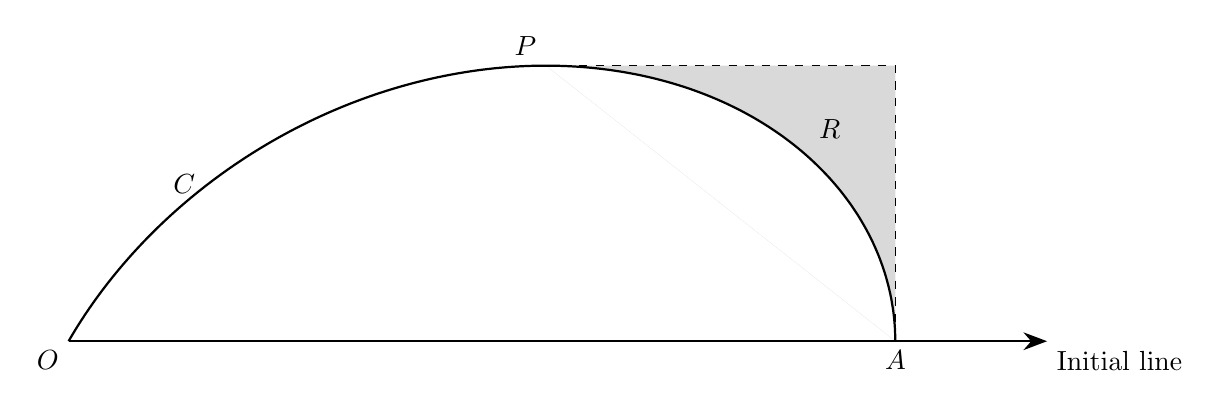
\begin{tikzpicture}[scale=3.5]
\def\thP{30}
\def\thMax{60}
\def\thC{50}
\pgfmathsetmacro{\rP}{1 + 2*cos(2*\thP)}
\pgfmathsetmacro{\xP}{\rP*cos(\thP)}
\pgfmathsetmacro{\yP}{\rP*sin(\thP)}
\coordinate (O) at (0,0);
\coordinate (A) at (3,0);
\coordinate (P) at (\xP,\yP);
\coordinate (T) at (3,\yP);
\coordinate (I) at (3.55,0);
\coordinate (CL) at ({(1 + 2*cos(2*\thC))*cos(\thC)},{(1 + 2*cos(2*\thC))*sin(\thC)});
\coordinate (Rlabel) at ($(A)!0.52!(P)+(0.42,0.25)$);

\fill[gray!30] (P) -- (T) -- (A)
  plot[smooth, samples=120, domain=0:\thP]
    ({(1 + 2*cos(2*\x))*cos(\x)},{(1 + 2*cos(2*\x))*sin(\x)})
  -- cycle;

\draw[-{Stealth[length=3mm]}, thick] (O) -- (I);
\draw[thick] plot[smooth, samples=200, domain=0:\thMax]
  ({(1 + 2*cos(2*\x))*cos(\x)},{(1 + 2*cos(2*\x))*sin(\x)});
\draw[dashed] (P) -- (T) -- (A);

\node[below left] at (O) {$O$};
\node[below] at (A) {$A$};
\node[above left] at (P) {$P$};
\node[above] at (CL) {$C$};
\node at (Rlabel) {$R$};
\node[below right] at (I) {Initial line};
\end{tikzpicture}
\end{figure}


The curve $C$ shown in the figure above has polar equation
\[
r = 1 + 2\cos 2\theta, \qquad 0 \leq \theta \leq \frac{\pi}{3}
\]
\\
At the point $P$ on $C$, the tangent to $C$ is parallel to the initial line. \\

\begin{enumerate}[label=\textbf{(\alph*)}]
  \item Show that $P$ has polar coordinates $\left(2, \dfrac{\pi}{6}\right)$. \marks{4} \\
\end{enumerate}
The point $A$ on $C$ has polar coordinates $(3, 0)$. \\

The finite region $R$, shown shaded in the figure above, is bounded by the arc $AP$ of $C$, the tangent to $C$ at $P$ and the line through $A$ parallel to $\theta = \frac{\pi}{2}$. \\
\begin{enumerate}[label=\textbf{(\alph*)}, resume]
  \item Find the exact area of $R$. \marks{9} \\
\end{enumerate}

\vspace*{10pt}

\begin{tcolorbox}[colback=white, colframe=scarlet, title={\textbf{Solution}}, breakable, grow to left by=6mm, grow to right by=10mm]
\begin{enumerate}[label=\textbf{(\alph*)}]
  \item Using
\[
x=r\cos\theta,\qquad y=r\sin\theta
\]
with
\[
r=1+2\cos 2\theta
\]
we have
\[
\frac{\mathrm{d}y}{\mathrm{d}x}=\frac{\frac{\mathrm{d}y}{\mathrm{d}\theta}}{\frac{\mathrm{d}x}{\mathrm{d}\theta}}
\]

Since the tangent is parallel to the initial line, it is horizontal, so
\[
\frac{\mathrm{d}y}{\mathrm{d}\theta}=0
\qquad \text{and} \qquad
\frac{\mathrm{d}x}{\mathrm{d}\theta}\neq 0
\]

First,
\[
\frac{\mathrm{d}r}{\mathrm{d}\theta}=-4\sin 2\theta
\]

Now
\begin{align*}
\frac{\mathrm{d}y}{\mathrm{d}\theta}
&=\frac{\mathrm{d}}{\mathrm{d}\theta}(r\sin\theta) \\
&=\frac{\mathrm{d}r}{\mathrm{d}\theta}\sin\theta+r\cos\theta \\
&=-4\sin 2\theta\sin\theta+(1+2\cos 2\theta)\cos\theta \\
&=-8\sin^2\theta\cos\theta+\bigl(1+2(1-2\sin^2\theta)\bigr)\cos\theta \\
&=-8\sin^2\theta\cos\theta+(3-4\sin^2\theta)\cos\theta \\
&=3\cos\theta(1-4\sin^2\theta)
\end{align*}

So
\[
3\cos\theta(1-4\sin^2\theta)=0
\]

For \(0\le \theta \le \frac{\pi}{3}\), we have \(\cos\theta>0\), so
\[
1-4\sin^2\theta=0
\]
Hence
\[
\sin\theta=\frac12
\]
and in the given interval this gives
\[
\theta=\frac{\pi}{6}
\]

Now find \(r\):
\[
r=1+2\cos\left(2\cdot \frac{\pi}{6}\right)
=1+2\cos\frac{\pi}{3}
=1+2\cdot \frac12
=2
\]

Also,
\[
\frac{\mathrm{d}x}{\mathrm{d}\theta}
=\frac{\mathrm{d}}{\mathrm{d}\theta}(r\cos\theta)
=\frac{\mathrm{d}r}{\mathrm{d}\theta}\cos\theta-r\sin\theta
\]
and at \(\theta=\frac{\pi}{6}\),
\[
\frac{\mathrm{d}x}{\mathrm{d}\theta}
=(-2\sqrt3)\cdot \frac{\sqrt3}{2}-2\cdot \frac12=-3-1=-4\neq 0
\]
so this does give a horizontal tangent.

Therefore \(P\) has polar coordinates
\[
\left(2,\frac{\pi}{6}\right)
\]

  \item Let \(Q\) be the point where the tangent at \(P\) meets the vertical line through \(A\).

From part (a),
\[
P=\left(2,\frac{\pi}{6}\right)
\]
so in Cartesian coordinates,
\[
P=\left(2\cos\frac{\pi}{6},\,2\sin\frac{\pi}{6}\right)=(\sqrt3,1)
\]

Also \(A=(3,0)\), since its polar coordinates are \((3,0)\).

The tangent at \(P\) is parallel to the initial line, so it is
\[
y=1
\]
The line through \(A\) parallel to \(\theta=\frac{\pi}{2}\) is vertical, so it is
\[
x=3
\]
Hence
\[
Q=(3,1)
\]

If the arc \(AP\) were replaced by the chord \(AP\), the region would be triangle \(AQP\). So
\[
\text{Area}(R)=\text{Area}(\triangle AQP)-\text{area between chord }AP\text{ and arc }AP
\]

First,
\[
AQ=1,\qquad QP=3-\sqrt3
\]
so
\[
\text{Area}(\triangle AQP)=\frac12(1)(3-\sqrt3)=\frac{3-\sqrt3}{2}
\]

Now find the area between the chord and the arc.

This is
\[
\text{Area of sector }OAP-\text{Area}(\triangle OAP)
\]

For the sector,
\[
\text{Area of sector }OAP=\frac12\int_0^{\pi/6} r^2\,\mathrm{d}\theta
=\frac12\int_0^{\pi/6}(1+2\cos 2\theta)^2\,\mathrm{d}\theta
\]

Expand the square:
\begin{align*}
(1+2\cos 2\theta)^2
&=1+4\cos 2\theta+4\cos^2 2\theta \\
&=1+4\cos 2\theta+2(1+\cos 4\theta) \\
&=3+4\cos 2\theta+2\cos 4\theta
\end{align*}

So
\begin{align*}
\text{Area of sector }OAP
&=\frac12\int_0^{\pi/6}\left(3+4\cos 2\theta+2\cos 4\theta\right)\,\mathrm{d}\theta \\
&=\frac12\left[3\theta+2\sin 2\theta+\frac12\sin 4\theta\right]_0^{\pi/6} \\
&=\frac12\left(\frac{\pi}{2}+2\sin\frac{\pi}{3}+\frac12\sin\frac{2\pi}{3}\right) \\
&=\frac12\left(\frac{\pi}{2}+2\cdot \frac{\sqrt3}{2}+\frac12\cdot \frac{\sqrt3}{2}\right) \\
&=\frac12\left(\frac{\pi}{2}+\sqrt3+\frac{\sqrt3}{4}\right) \\
&=\frac{\pi}{4}+\frac{5\sqrt3}{8}
\end{align*}

For triangle \(OAP\),
\[
OA=3,\qquad OP=2,\qquad \angle AOP=\frac{\pi}{6}
\]
so
\[
\text{Area}(\triangle OAP)=\frac12\cdot 3\cdot 2\cdot \sin\frac{\pi}{6}=\frac32
\]

Hence the area between chord \(AP\) and arc \(AP\) is
\[
\left(\frac{\pi}{4}+\frac{5\sqrt3}{8}\right)-\frac32
\]

Therefore
\begin{align*}
\text{Area}(R)
&=\frac{3-\sqrt3}{2}-\left[\left(\frac{\pi}{4}+\frac{5\sqrt3}{8}\right)-\frac32\right] \\
&=\frac{3-\sqrt3}{2}+\frac32-\frac{\pi}{4}-\frac{5\sqrt3}{8} \\
&=3-\frac{\pi}{4}-\frac{9\sqrt3}{8}
\end{align*}

So the exact area of \(R\) is
\[
3-\frac{\pi}{4}-\frac{9\sqrt3}{8}
\]
equivalently
\[
\frac{24-2\pi-9\sqrt3}{8}
\]
\end{enumerate}
\end{tcolorbox}


\newpage

% ---- Question 2 ----
\questionitem

The curve $C$ has polar equation
\[
r = 2\sin 3\theta, \qquad 0 \leq \theta \leq \frac{\pi}{3}
\]
\\
At the non-pole point $P$ on $C$, the tangent to $C$ is parallel to the initial line. \\

Given that $O$ is the pole, find the exact length of the line $OP$. \marks{7}

\vspace*{10pt}

\begin{tcolorbox}[colback=white, colframe=scarlet, title={\textbf{Solution}}, breakable, grow to left by=6mm, grow to right by=10mm]
For a polar curve,
\[
x=r\cos\theta,\qquad y=r\sin\theta,\qquad \frac{\mathrm{d}y}{\mathrm{d}x}=\frac{\mathrm{d}y/\mathrm{d}\theta}{\mathrm{d}x/\mathrm{d}\theta}
\]

A tangent parallel to the initial line is horizontal, so its gradient is \(0\). Hence we require
\[
\frac{\mathrm{d}y}{\mathrm{d}\theta}=0
\]
with \(\dfrac{\mathrm{d}x}{\mathrm{d}\theta}\neq 0\).

Here
\[
r=2\sin 3\theta
\]
so
\[
\frac{\mathrm{d}r}{\mathrm{d}\theta}=6\cos 3\theta
\]

Now
\[
y=r\sin\theta
\]
so, by the product rule,
\begin{align*}
\frac{\mathrm{d}y}{\mathrm{d}\theta}
&=\frac{\mathrm{d}r}{\mathrm{d}\theta}\sin\theta+r\cos\theta \\
&=6\cos 3\theta \sin\theta+2\sin 3\theta \cos\theta
\end{align*}

Set this equal to \(0\):
\[
6\cos 3\theta \sin\theta+2\sin 3\theta \cos\theta=0
\]

Divide by \(2\):
\[
3\cos 3\theta \sin\theta+\sin 3\theta \cos\theta=0
\]

Using the product-to-sum identities,
\[
\sin\theta\cos 3\theta=\frac12(\sin 4\theta-\sin 2\theta),
\qquad
\cos\theta\sin 3\theta=\frac12(\sin 4\theta+\sin 2\theta)
\]

So
\begin{align*}
0
&=3\cdot \frac12(\sin 4\theta-\sin 2\theta)+\frac12(\sin 4\theta+\sin 2\theta) \\
&=\frac12\bigl(4\sin 4\theta-2\sin 2\theta\bigr)
\end{align*}

Hence
\[
2\sin 4\theta-\sin 2\theta=0
\]

Using \(\sin 4\theta=2\sin 2\theta \cos 2\theta\),
\begin{align*}
0&=2(2\sin 2\theta \cos 2\theta)-\sin 2\theta \\
&=\sin 2\theta(4\cos 2\theta-1)
\end{align*}

At a non-pole point on this curve, \(0<\theta<\frac{\pi}{3}\), so \(0<2\theta<\frac{2\pi}{3}\), and therefore \(\sin 2\theta\neq 0\). Thus
\[
4\cos 2\theta-1=0
\]
so
\[
\cos 2\theta=\frac14
\]

Now use \(\cos 2\theta=2\cos^2\theta-1\):
\begin{align*}
2\cos^2\theta-1&=\frac14 \\
2\cos^2\theta&=\frac54 \\
\cos^2\theta&=\frac58
\end{align*}

Therefore
\[
\sin^2\theta=1-\frac58=\frac38
\]

Since \(0<\theta<\frac{\pi}{3}\), both \(\sin\theta\) and \(\cos\theta\) are positive, so
\[
\sin\theta=\sqrt{\frac38}=\frac{\sqrt6}{4}
\]

Now
\[
r=2\sin 3\theta
\]
and using \(\sin 3\theta=3\sin\theta-4\sin^3\theta\),
\begin{align*}
r
&=2\left(3\cdot \frac{\sqrt6}{4}-4\left(\frac{\sqrt6}{4}\right)^3\right) \\
&=2\left(\frac{3\sqrt6}{4}-4\cdot \frac{6\sqrt6}{64}\right) \\
&=2\left(\frac{3\sqrt6}{4}-\frac{3\sqrt6}{8}\right) \\
&=2\left(\frac{3\sqrt6}{8}\right) \\
&=\frac{3\sqrt6}{4}
\end{align*}

Finally, check that this really is a horizontal tangent:
\begin{align*}
\frac{\mathrm{d}x}{\mathrm{d}\theta}
&=\frac{\mathrm{d}r}{\mathrm{d}\theta}\cos\theta-r\sin\theta \\
&=6\cos 3\theta\cos\theta-2\sin 3\theta\sin\theta \\
&=-3\neq 0
\end{align*}

So the tangent is genuinely parallel to the initial line.

Hence the exact length of \(OP\) is
\[
OP=r=\frac{3\sqrt6}{4}
\]
\end{tcolorbox}


\newpage

% ---- Question 3 ----
\questionitem

\begin{figure}[H]
    \centering
\begin{tikzpicture}[scale=1.5]
\def\rA{2}
\def\k{0.60}
\def\thP{0.82}
\pgfmathsetmacro{\rP}{\rA*exp(\k*\thP)}
\pgfmathsetmacro{\xP}{\rP*cos(deg(\thP))}
\pgfmathsetmacro{\yP}{\rP*sin(deg(\thP))}
\pgfmathsetmacro{\dx}{\rP*(\k*cos(deg(\thP)) - sin(deg(\thP)))}
\pgfmathsetmacro{\dy}{\rP*(\k*sin(deg(\thP)) + cos(deg(\thP)))}
\pgfmathsetmacro{\tT}{-\yP/\dy}
\pgfmathsetmacro{\xT}{\xP + \tT*\dx}
\pgfmathsetmacro{\tQ}{0.75}
\pgfmathsetmacro{\xQ}{\xP + \tQ*\dx}
\pgfmathsetmacro{\yQ}{\yP + \tQ*\dy}
\pgfmathsetmacro{\xEnd}{\xT + 0.55}
\pgfmathsetmacro{\thC}{1.3}
\pgfmathsetmacro{\rC}{\rA*exp(\k*\thC)}
\pgfmathsetmacro{\xC}{\rC*cos(deg(\thC))}
\pgfmathsetmacro{\yC}{\rC*sin(deg(\thC))}

\coordinate (O) at (0,0);
\coordinate (I) at (1,0);
\coordinate (A) at (\rA,0);
\coordinate (P) at (\xP,\yP);
\coordinate (T) at (\xT,0);
\coordinate (Q) at (\xQ,\yQ);
\coordinate (CLabel) at (\xC,\yC);

\draw[thick] (O) -- (\xEnd,0);
\draw[dashed] (O) -- (P);
\draw[thick] (Q) -- (T);
\draw[thick, black] plot[smooth, samples=160, domain=0:1.30, variable=\t]
  ({\rA*exp(\k*\t)*cos(deg(\t))},{\rA*exp(\k*\t)*sin(deg(\t))});

\pic["$\theta$", draw, angle radius=5mm, angle eccentricity=1.35]
  {angle=I--O--P};

\node[below left] at (O) {$O$};
\node[below] at (A) {$A$};
\node[right] at (P) {$P$};
\node[below] at (T) {$T$};
\node[above] at (Q) {$Q$};
\node[below left] at (CLabel) {$C$};
\draw[-{Stealth[length=3mm]}, thick] (O) -- (4.5, 0)
  node[pos=0.95, below] {Initial line};
\end{tikzpicture}
\end{figure}


The diagram shows part of a spiral $C$. \\

The point $P$ has polar coordinates $(r, \theta)$, where $0 \leq \theta \leq \frac{\pi}{2}$. \\

The tangent at $P$ is the line $TPQ$. The point $A$ lies on $C$ and on the initial line, with $OA = 2$. \\

Let $\psi$ be the angle that $TPQ$ makes with the initial line. \\

\begin{enumerate}[label=\textbf{(\alph*)}]
  \item By expressing the Cartesian coordinates of $P$ in terms of $r$ and $\theta$, show that
  \[
  \tan \psi = \frac{\frac{\mathrm{d}r}{\mathrm{d}\theta}\sin\theta + r\cos\theta}{\frac{\mathrm{d}r}{\mathrm{d}\theta}\cos\theta - r\sin\theta}
  \]
  \marks[-30pt]{4}
  \item The spiral is equiangular: at every point $P$, the acute angle between $OP$ and $TPQ$ is a constant $\alpha$, where $0 < \alpha < \frac{\pi}{2}$. \\

  Use the result of part (a) to show that the polar equation of $C$ is
  \[
  r = 2e^{(\cot \alpha)\theta}
  \]
  \marks[-20pt]{7}
\end{enumerate}

\vspace*{10pt}

\begin{tcolorbox}[colback=white, colframe=scarlet, title={\textbf{Solution}}, breakable, grow to left by=6mm, grow to right by=10mm]
\begin{enumerate}[label=\textbf{(\alph*)}]
  \item Let the Cartesian coordinates of \(P\) be \((x,y)\).  
  Since \(P\) has polar coordinates \((r,\theta)\),
  \[
  x=r\cos\theta,\qquad y=r\sin\theta
  \]

  Differentiate both with respect to \(\theta\):
  \begin{align*}
  \frac{\mathrm{d}x}{\mathrm{d}\theta}
  &= \frac{\mathrm{d}r}{\mathrm{d}\theta}\cos\theta-r\sin\theta \\
  \frac{\mathrm{d}y}{\mathrm{d}\theta}
  &= \frac{\mathrm{d}r}{\mathrm{d}\theta}\sin\theta+r\cos\theta
  \end{align*}

  The angle \(\psi\) is the angle the tangent makes with the initial line, so
  \[
  \tan\psi=\frac{\mathrm{d}y}{\mathrm{d}x}
  \]

  Using
  \[
  \frac{\mathrm{d}y}{\mathrm{d}x}=\frac{\frac{\mathrm{d}y}{\mathrm{d}\theta}}{\frac{\mathrm{d}x}{\mathrm{d}\theta}}
  \]
  gives
  \[
  \tan\psi
  =\frac{\frac{\mathrm{d}r}{\mathrm{d}\theta}\sin\theta+r\cos\theta}{\frac{\mathrm{d}r}{\mathrm{d}\theta}\cos\theta-r\sin\theta}
  \]

  So
  \[
  \tan \psi = \frac{\frac{\mathrm{d}r}{\mathrm{d}\theta}\sin\theta + r\cos\theta}{\frac{\mathrm{d}r}{\mathrm{d}\theta}\cos\theta - r\sin\theta}
  \]
  as required.

  \item Let
  \[
  r'=\frac{\mathrm{d}r}{\mathrm{d}\theta}
  \]

  From part (a),
  \[
  \tan\psi=\frac{r'\sin\theta+r\cos\theta}{r'\cos\theta-r\sin\theta}
  \]

  Divide top and bottom by \(r'\cos\theta\):
  \begin{align*}
  \tan\psi
  &=\frac{\tan\theta+\frac{r}{r'}}{1-\tan\theta\frac{r}{r'}}
  \end{align*}

  Now let \(\beta\) be defined by
  \[
  \tan\beta=\frac{r}{r'}
  \]

  Then
  \begin{align*}
  \tan\psi
  &=\frac{\tan\theta+\tan\beta}{1-\tan\theta\tan\beta} \\
  &=\tan(\theta+\beta)
  \end{align*}

  So the angle between \(OP\) and the tangent is \(\beta\).

  But the spiral is equiangular, so this acute angle is the constant \(\alpha\). Hence
  \[
  \beta=\alpha
  \]
  and therefore
  \[
  \tan\alpha=\frac{r}{r'}
  \]

  So
  \begin{align*}
  \frac{r}{\frac{\mathrm{d}r}{\mathrm{d}\theta}} &= \tan\alpha \\
  \frac{\mathrm{d}r}{\mathrm{d}\theta} &= r\cot\alpha
  \end{align*}

  This is a separable differential equation:
  \[
  \frac{1}{r}\,\mathrm{d}r=\cot\alpha\,\mathrm{d}\theta
  \]

  Integrating,
  \begin{align*}
  \int \frac{1}{r}\,\mathrm{d}r &= \int \cot\alpha\,\mathrm{d}\theta \\
  \ln r &= (\cot\alpha)\theta + c
  \end{align*}

  At the point \(A\), the curve is on the initial line and \(OA=2\), so
  \[
  \theta=0,\qquad r=2
  \]

  Substitute into the equation:
  \begin{align*}
  \ln 2 &= (\cot\alpha)(0)+c \\
  c&=\ln 2
  \end{align*}

  Hence
  \begin{align*}
  \ln r &= (\cot\alpha)\theta+\ln 2 \\
  r &= 2e^{(\cot\alpha)\theta}
  \end{align*}

  Therefore the polar equation of \(C\) is
  \[
  r = 2e^{(\cot \alpha)\theta}
  \]
\end{enumerate}
\end{tcolorbox}


\newpage

% ---- Question 4 ----
\questionitem

\begin{figure}[H]
    \centering
\begin{tikzpicture}[scale=1.5]
\def\axislen{5.2}
\def\labang{60}
\draw[-{Stealth[length=3mm]}, thick] (0,0) -- (\axislen,0) node[pos=0.95, below] {Initial line};
\draw[thick, black]
  plot[smooth, samples=300, domain=-180:180]
    ({2*(1+cos(\x))*cos(\x)},{2*(1+cos(\x))*sin(\x)});
\coordinate (L) at ({2*(1+cos(\labang))*cos(\labang)},{2*(1+cos(\labang))*sin(\labang)});
\node[above right] at (L) {$C_1$};
\node[below] at (0,0) {$O$};
\end{tikzpicture}
\end{figure}


The diagram shows the sketch of a curve $C_1$. \\

The polar equation of the curve $C_1$ is
\[
r = 2(1 + \cos \theta), \qquad -\pi \leq \theta \leq \pi
\]
\begin{enumerate}[label=\textbf{(\alph*)}]
  \item Find the area of the region bounded by the curve $C_1$. \marks{5} \\
  \item The curve $C_2$ whose polar equation is
  \[
  r = \sin \theta, \qquad 0 \leq \theta \leq \pi
  \]
  intersects the curve $C_1$ at the pole $O$ and at the point $A$. The straight line drawn through $A$ perpendicular to the initial line intersects the part of $C_1$ above the initial line again at the point $B$. \\
  \begin{enumerate}[label=(\roman*)]
    \item Find the polar coordinates of $A$. \marks{4}
    \item Show that the length of $OB$ is $\dfrac{6}{5}$. \marks{6}
    \item Find the length of $AB$, giving your answer to three significant figures. \marks{3}
  \end{enumerate}
\end{enumerate}

\vspace*{10pt}

\begin{tcolorbox}[colback=white, colframe=scarlet, title={\textbf{Solution}}, breakable, grow to left by=6mm, grow to right by=10mm]
\begin{enumerate}[label=\textbf{(\alph*)}]
  \item Using the polar area formula,
\[
\text{Area}=\frac12\int_{-\pi}^{\pi} r^2\,\mathrm{d}\theta
\]

Here \(r=2(1+\cos\theta)\), so
\[
\text{Area}=\frac12\int_{-\pi}^{\pi}\bigl(2(1+\cos\theta)\bigr)^2\,\mathrm{d}\theta
=2\int_{-\pi}^{\pi}(1+2\cos\theta+\cos^2\theta)\,\mathrm{d}\theta
\]

Using \(\cos^2\theta=\dfrac{1+\cos 2\theta}{2}\),
\[
\text{Area}
=2\int_{-\pi}^{\pi}\left(1+2\cos\theta+\frac{1+\cos2\theta}{2}\right)\,\mathrm{d}\theta
\]

\[
=2\int_{-\pi}^{\pi}\left(\frac32+2\cos\theta+\frac12\cos2\theta\right)\,\mathrm{d}\theta
\]

\[
=2\left[\frac32\theta+2\sin\theta+\frac14\sin2\theta\right]_{-\pi}^{\pi}
\]

At \(\theta=\pi\) and \(\theta=-\pi\), the sine terms are \(0\), so
\[
\text{Area}
=2\left(\frac32\pi-\left(-\frac32\pi\right)\right)
=2(3\pi)
=6\pi
\]

Hence the area of the region bounded by \(C_1\) is \(6\pi\).

  \item
\begin{enumerate}[label=(\roman*)]
\item Since both curves have \(r\ge 0\) on the given ranges, any intersection away from the pole must occur for the same value of \(\theta\).

So we solve
\[
2(1+\cos\theta)=\sin\theta
\]

Squaring both sides,
\[
4(1+\cos\theta)^2=\sin^2\theta
\]

Using \(\sin^2\theta=1-\cos^2\theta\),
\[
4(1+2\cos\theta+\cos^2\theta)=1-\cos^2\theta
\]

\[
4+8\cos\theta+4\cos^2\theta=1-\cos^2\theta
\]

\[
5\cos^2\theta+8\cos\theta+3=0
\]

\[
(5\cos\theta+3)(\cos\theta+1)=0
\]

So
\[
\cos\theta=-\frac35 \quad \text{or} \quad \cos\theta=-1
\]

The value \(\cos\theta=-1\) gives \(\theta=\pi\), and then \(r=\sin\pi=0\), which is the pole \(O\).

Therefore point \(A\) corresponds to
\[
\cos\theta=-\frac35
\]

Since \(0\le \theta\le \pi\), we have \(\sin\theta>0\), so
\[
\sin\theta=\sqrt{1-\left(-\frac35\right)^2}=\sqrt{1-\frac{9}{25}}=\frac45
\]

Hence
\[
r=\sin\theta=\frac45
\]

So the polar coordinates of \(A\) are
\[
\left(\frac45,\ \arccos\left(-\frac35\right)\right)
\]

Equivalently, \(\theta\approx 126.9^\circ\).

\item The line through \(A\) perpendicular to the initial line is a vertical line, so points \(A\) and \(B\) have the same \(x\)-coordinate.

For \(A\),
\[
x_A=r\cos\theta=\frac45\cdot\left(-\frac35\right)=-\frac{12}{25}
\]

For a general point on \(C_1\),
\[
r=2(1+\cos\theta)
\]
so
\[
x=r\cos\theta=2\cos\theta(1+\cos\theta)
\]

At point \(B\), \(x=x_A\), so
\[
2\cos\theta(1+\cos\theta)=-\frac{12}{25}
\]

Let \(c=\cos\theta\). Then
\[
2c(1+c)=-\frac{12}{25}
\]

\[
50c^2+50c=-12
\]

\[
25c^2+25c+6=0
\]

\[
(5c+3)(5c+2)=0
\]

So
\[
c=-\frac35 \quad \text{or} \quad c=-\frac25
\]

The root \(c=-\frac35\) corresponds to \(A\), so for \(B\),
\[
\cos\theta=-\frac25
\]

Hence
\[
r_B=2\left(1-\frac25\right)=2\cdot\frac35=\frac65
\]

Since \(OB\) is the distance from the pole to \(B\),
\[
OB=\frac65
\]

So the length of \(OB\) is \(\dfrac65\).

\item Since \(AB\) is vertical, its length is the difference between the \(y\)-coordinates of \(B\) and \(A\).

For \(A\),
\[
y_A=r\sin\theta=\frac45\cdot\frac45=\frac{16}{25}
\]

For \(B\), we have \(\cos\theta=-\frac25\), and \(B\) is above the initial line, so
\[
\sin\theta=\sqrt{1-\left(-\frac25\right)^2}
=\sqrt{1-\frac{4}{25}}
=\frac{\sqrt{21}}{5}
\]

Therefore
\[
y_B=r\sin\theta=\frac65\cdot\frac{\sqrt{21}}{5}
=\frac{6\sqrt{21}}{25}
\]

So
\[
AB=y_B-y_A=\frac{6\sqrt{21}}{25}-\frac{16}{25}
=\frac{6\sqrt{21}-16}{25}
\]

\[
AB\approx 0.460
\]

Hence
\[
AB=\frac{6\sqrt{21}-16}{25}\approx 0.460
\]
to three significant figures.
\end{enumerate}
\end{enumerate}
\end{tcolorbox}


\newpage

% ---- Question 5 ----
\questionitem

The curve $C$ has polar equation
\[
r = 3\sin 2\theta, \qquad 0 \leq \theta \leq \frac{\pi}{2}
\]
\\
At the non-pole point $P$ on $C$, the tangent to $C$ is perpendicular to the initial line. \\

Given that $O$ is the pole, find the exact length of the line $OP$. \marks{7}

\vspace*{10pt}
\begin{tcolorbox}[colback=white, colframe=scarlet, title={\textbf{Solution}}, breakable, grow to left by=6mm, grow to right by=10mm]
For a polar curve,
\[
x=r\cos\theta,\qquad y=r\sin\theta
\]
so
\[
\frac{\mathrm{d}y}{\mathrm{d}x}
=
\frac{\dfrac{\mathrm{d}y}{\mathrm{d}\theta}}{\dfrac{\mathrm{d}x}{\mathrm{d}\theta}}
=
\frac{r'\sin\theta+r\cos\theta}{r'\cos\theta-r\sin\theta}
\]

A tangent perpendicular to the initial line is vertical, so \(\dfrac{\mathrm{d}y}{\mathrm{d}x}\) is undefined. Therefore
\[
r'\cos\theta-r\sin\theta=0
\]
with \(r'\sin\theta+r\cos\theta\neq 0\)

Given
\[
r=3\sin 2\theta
\]
we have
\[
r'=6\cos 2\theta
\]

Substituting into the vertical tangent condition gives
\[
6\cos 2\theta\cos\theta-3\sin 2\theta\sin\theta=0
\]

Now use
\[
\cos 2\theta=\cos^2\theta-\sin^2\theta,
\qquad
\sin 2\theta=2\sin\theta\cos\theta
\]
Then
\begin{align*}
6(\cos^2\theta-\sin^2\theta)\cos\theta-3(2\sin\theta\cos\theta)\sin\theta&=0\\
6(\cos^2\theta-\sin^2\theta)\cos\theta-6\sin^2\theta\cos\theta&=0\\
6\cos\theta(\cos^2\theta-2\sin^2\theta)&=0
\end{align*}

Using \(\sin^2\theta=1-\cos^2\theta\),
\begin{align*}
6\cos\theta\bigl(\cos^2\theta-2(1-\cos^2\theta)\bigr)&=0\\
6\cos\theta(3\cos^2\theta-2)&=0
\end{align*}

Since \(P\) is a non-pole point and \(0\leq \theta \leq \dfrac{\pi}{2}\), we must have
\[
0<\theta<\frac{\pi}{2}
\]
so \(\cos\theta\neq 0\)

Hence
\[
3\cos^2\theta-2=0
\]
so
\[
\cos^2\theta=\frac{2}{3}
\]

Also
\[
\sin^2\theta=1-\frac{2}{3}=\frac{1}{3}
\]

Because \(0<\theta<\dfrac{\pi}{2}\), both sine and cosine are positive, so
\[
\cos\theta=\sqrt{\frac{2}{3}},
\qquad
\sin\theta=\frac{1}{\sqrt{3}}
\]

Now
\begin{align*}
r&=3\sin 2\theta\\
&=3(2\sin\theta\cos\theta)\\
&=6\cdot \frac{1}{\sqrt{3}}\cdot \sqrt{\frac{2}{3}}\\
&=2\sqrt{2}
\end{align*}

Finally, check that the numerator is non-zero:
\begin{align*}
r'\sin\theta+r\cos\theta
&=6\cos 2\theta\sin\theta+3\sin 2\theta\cos\theta\\
&=6\left(\frac{1}{3}\right)\left(\frac{1}{\sqrt{3}}\right)
+3\left(\frac{2\sqrt{2}}{3}\right)\left(\sqrt{\frac{2}{3}}\right)\\
&=\frac{2}{\sqrt{3}}+\frac{4}{\sqrt{3}}\\
&=\frac{6}{\sqrt{3}}=2\sqrt{3}\neq 0
\end{align*}

So the tangent is genuinely perpendicular to the initial line, and since \(OP=r\),
\[
OP=2\sqrt{2}
\]
\end{tcolorbox}


\newpage

% ---- Question 6 ----
\questionitem

\begin{figure}[H]
    \centering
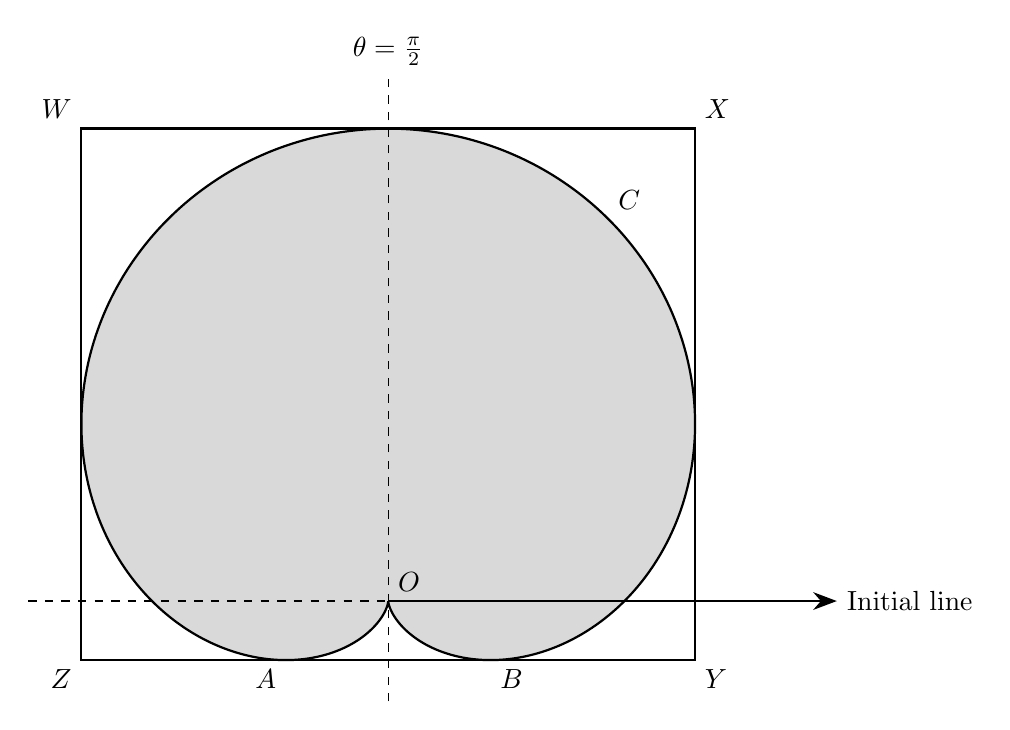
\begin{tikzpicture}[scale=1.5]
\def\a{2}
\pgfmathsetmacro{\xleft}{-3*sqrt(3)*\a/4}
\pgfmathsetmacro{\xright}{3*sqrt(3)*\a/4}
\pgfmathsetmacro{\ytop}{2*\a}
\pgfmathsetmacro{\ybottom}{-\a/4}
\pgfmathsetmacro{\xab}{sqrt(3)*\a/4}

\coordinate (O) at (0,0);
\coordinate (W) at (\xleft,\ytop);
\coordinate (X) at (\xright,\ytop);
\coordinate (Y) at (\xright,\ybottom);
\coordinate (Z) at (\xleft,\ybottom);
\coordinate (A) at (-\xab,\ybottom);
\coordinate (B) at (\xab,\ybottom);
\coordinate (Clbl) at ({\a*(1+sin(60))*cos(60)},{\a*(1+sin(60))*sin(60)});

\fill[gray!30]
  plot[smooth, samples=300, domain=-1.570796:4.712389]
    ({\a*(1+sin(deg(\x)))*cos(deg(\x))},{\a*(1+sin(deg(\x)))*sin(deg(\x))})
  -- cycle;

\draw[thick] (W) -- (X) -- (Y) -- (Z) -- cycle;
\draw[dashed] (\xleft-0.45,0) -- (O);
\draw[dashed] (0,\ybottom-0.35) -- (0,\ytop+0.45);
\draw[-{Stealth[length=3mm]}, thick] (O) -- (\xright+1.2,0) node[right] {Initial line};

\draw[thick]
  plot[smooth, samples=300, domain=-1.570796:4.712389]
    ({\a*(1+sin(deg(\x)))*cos(deg(\x))},{\a*(1+sin(deg(\x)))*sin(deg(\x))});

\node[above left] at (W) {$W$};
\node[above right] at (X) {$X$};
\node[below right] at (Y) {$Y$};
\node[below left] at (Z) {$Z$};
\node[below left] at (A) {$A$};
\node[below right] at (B) {$B$};
\node[above right] at (O) {$O$};
\node[above] at (0,\ytop+0.45) {$\theta=\frac{\pi}{2}$};
\node[above right] at (Clbl) {$C$};
\end{tikzpicture}
\end{figure}


The figure shows a sketch of the cardioid $C$ with equation
\[
r = a(1 + \sin \theta), \qquad 0 \leq \theta < 2\pi
\]
\\
Also shown are the tangents to $C$ that are parallel and perpendicular to the initial line. These tangents form a rectangle $WXYZ$. \\

\begin{enumerate}[label=\textbf{(\alph*)}]
  \item Find the area of the finite region, shaded in the figure, enclosed by $C$. \marks{6} \\
  \item Find the values of $\theta$ for which the tangent to $C$ is parallel to the initial line. Hence find the polar coordinates of the points $A$ and $B$, where $ZY$ touches $C$. \marks{6} \\
  \item Hence show that the length of $WZ$ is $\dfrac{9a}{4}$. \marks{2} \\
\end{enumerate}
Given that the length of $WX$ is $\dfrac{3\sqrt{3}a}{2}$ \\
\begin{enumerate}[label=\textbf{(\alph*)}, resume]
  \item find the area of the rectangle $WXYZ$. \marks{2} \\
\end{enumerate}
A logo is modelled by the cardioid $C$, where $a = 8\,\text{cm}$. The logo is cut from the rectangular card $WXYZ$, shown in the figure. \\
\begin{enumerate}[label=\textbf{(\alph*)}, resume]
  \item Find a numerical value for the area of card wasted in making the logo. \marks{3} \\
\end{enumerate}

\vspace*{10pt}

\begin{tcolorbox}[colback=white, colframe=scarlet, title={\textbf{Solution}}, breakable, grow to left by=6mm, grow to right by=10mm]
\begin{enumerate}[label=\textbf{(\alph*)}]
  \item For a polar curve \(r=f(\theta)\), the area enclosed is
  \[
  \frac12\int r^2\,\mathrm{d}\theta
  \]

  Here \(r=a(1+\sin\theta)\), and \(0\le \theta<2\pi\) traces the whole cardioid once, so
  \begin{align*}
  \text{Area}
  &= \frac12\int_0^{2\pi} a^2(1+\sin\theta)^2\,\mathrm{d}\theta \\
  &= \frac{a^2}{2}\int_0^{2\pi}\left(1+2\sin\theta+\sin^2\theta\right)\,\mathrm{d}\theta
  \end{align*}

  Using \(\sin^2\theta=\dfrac{1-\cos 2\theta}{2}\),
  \begin{align*}
  \text{Area}
  &= \frac{a^2}{2}\int_0^{2\pi}\left(1+2\sin\theta+\frac{1-\cos 2\theta}{2}\right)\,\mathrm{d}\theta \\
  &= \frac{a^2}{2}\int_0^{2\pi}\left(\frac32+2\sin\theta-\frac12\cos 2\theta\right)\,\mathrm{d}\theta \\
  &= \frac{a^2}{2}\left[\frac32\theta-2\cos\theta-\frac14\sin 2\theta\right]_0^{2\pi} \\
  &= \frac{a^2}{2}\left(3\pi\right)
  \end{align*}

  Therefore the area enclosed by \(C\) is
  \[
  \frac{3\pi a^2}{2}
  \]

  \item Let
  \[
  x=r\cos\theta,\qquad y=r\sin\theta
  \]
  with
  \[
  r=a(1+\sin\theta),\qquad \frac{\mathrm{d}r}{\mathrm{d}\theta}=a\cos\theta
  \]

  Also,
  \[
  \frac{\mathrm{d}y}{\mathrm{d}x}
  =
  \frac{\frac{\mathrm{d}y}{\mathrm{d}\theta}}{\frac{\mathrm{d}x}{\mathrm{d}\theta}}
  \]

  A tangent parallel to the initial line is horizontal, so we need
  \[
  \frac{\mathrm{d}y}{\mathrm{d}\theta}=0
  \]
  with \(\frac{\mathrm{d}x}{\mathrm{d}\theta}\neq 0\).

  Now
  \begin{align*}
  \frac{\mathrm{d}y}{\mathrm{d}\theta}
  &= \frac{\mathrm{d}}{\mathrm{d}\theta}(r\sin\theta) \\
  &= \frac{\mathrm{d}r}{\mathrm{d}\theta}\sin\theta+r\cos\theta \\
  &= a\cos\theta\sin\theta+a(1+\sin\theta)\cos\theta \\
  &= a\cos\theta(1+2\sin\theta)
  \end{align*}

  So
  \[
  a\cos\theta(1+2\sin\theta)=0
  \]

  Hence either
  \[
  \cos\theta=0
  \quad\text{or}\quad
  1+2\sin\theta=0
  \]

  From \(\cos\theta=0\),
  \[
  \theta=\frac{\pi}{2},\ \frac{3\pi}{2}
  \]

  From \(1+2\sin\theta=0\),
  \[
  \sin\theta=-\frac12
  \]
  so
  \[
  \theta=\frac{7\pi}{6},\ \frac{11\pi}{6}
  \]

  At \(\theta=\dfrac{3\pi}{2}\),
  \[
  r=a(1+\sin\tfrac{3\pi}{2})=a(1-1)=0
  \]
  so this is the cusp at the pole, not a smooth horizontal tangent.

  Therefore the values of \(\theta\) for which the tangent is parallel to the initial line are
  \[
  \theta=\frac{\pi}{2},\ \frac{7\pi}{6},\ \frac{11\pi}{6}
  \]

  The line \(ZY\) is the lower horizontal tangent, so it touches \(C\) at the two lower points, where
  \[
  \theta=\frac{7\pi}{6},\ \frac{11\pi}{6}
  \]

  At each of these,
  \[
  r=a\left(1+\sin\theta\right)=a\left(1-\frac12\right)=\frac a2
  \]

  Hence the polar coordinates are
  \[
  A\left(\frac a2,\frac{7\pi}{6}\right),
  \qquad
  B\left(\frac a2,\frac{11\pi}{6}\right)
  \]

  \item From part (b), the upper horizontal tangent occurs at \(\theta=\dfrac{\pi}{2}\).

  Then
  \[
  r=a(1+\sin\tfrac{\pi}{2})=2a
  \]
  so its \(y\)-coordinate is
  \[
  y=r\sin\theta=2a\cdot 1=2a
  \]

  The lower horizontal tangent touches at \(A\) and \(B\), where \(r=\dfrac a2\) and \(\theta=\dfrac{7\pi}{6}\) or \(\dfrac{11\pi}{6}\), so
  \[
  y=\frac a2\sin\frac{7\pi}{6}=\frac a2\left(-\frac12\right)=-\frac a4
  \]

  Therefore the vertical distance between these tangents is
  \[
  WZ=2a-\left(-\frac a4\right)=\frac{9a}{4}
  \]

  So
  \[
  WZ=\frac{9a}{4}
  \]

  \item The area of the rectangle is
  \[
  \text{Area} = WX\times WZ
  \]

  Given
  \[
  WX=\frac{3\sqrt3\,a}{2}
  \qquad\text{and}\qquad
  WZ=\frac{9a}{4}
  \]
  we get
  \begin{align*}
  \text{Area}
  &= \frac{3\sqrt3\,a}{2}\times \frac{9a}{4} \\
  &= \frac{27\sqrt3\,a^2}{8}
  \end{align*}

  Therefore the area of rectangle \(WXYZ\) is
  \[
  \frac{27\sqrt3\,a^2}{8}
  \]

  \item When \(a=8\),
  \begin{align*}
  \text{Area of rectangle}
  &= \frac{27\sqrt3\,a^2}{8} \\
  &= \frac{27\sqrt3\cdot 8^2}{8} \\
  &= 216\sqrt3 \ \text{cm}^2
  \end{align*}

  From part (a),
  \begin{align*}
  \text{Area of cardioid}
  &= \frac{3\pi a^2}{2} \\
  &= \frac{3\pi\cdot 8^2}{2} \\
  &= 96\pi \ \text{cm}^2
  \end{align*}

  So the wasted area is
  \begin{align*}
  216\sqrt3-96\pi \ \text{cm}^2
  \end{align*}

  Numerically,
  \[
  216\sqrt3-96\pi \approx 72.5
  \]

  Therefore the area of card wasted is
  \[
  216\sqrt3-96\pi\ \text{cm}^2 \approx 72.5\ \text{cm}^2
  \]
\end{enumerate}
\end{tcolorbox}


\newpage

% ---- Question 7 ----
\questionitem

\begin{figure}[H]
    \centering
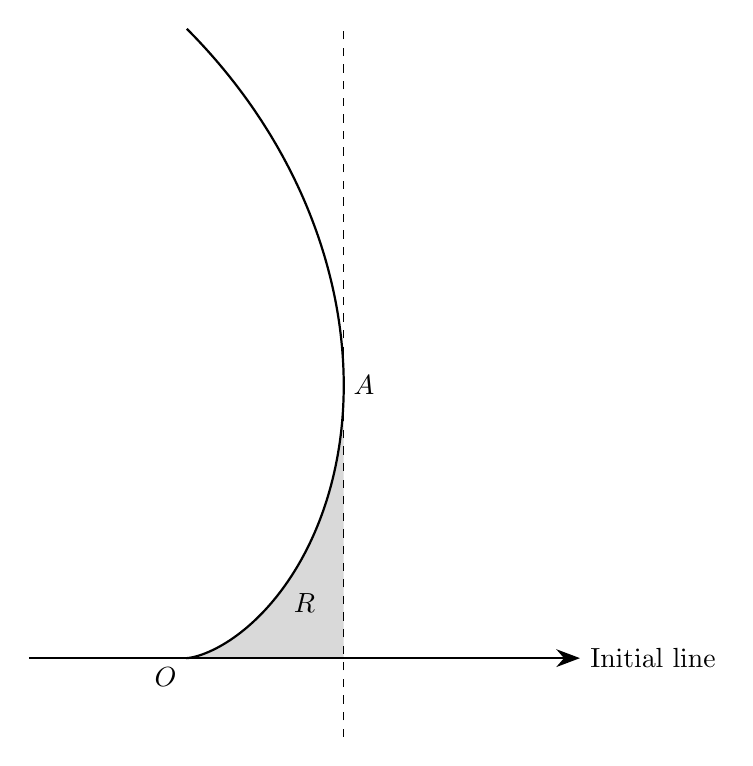
\begin{tikzpicture}[scale=2]
\pgfmathsetmacro{\thA}{pi/3}
\pgfmathsetmacro{\thmax}{pi/2}
\pgfmathsetmacro{\xA}{1}
\pgfmathsetmacro{\yA}{sqrt(3)}

\coordinate (O) at (0,0);
\coordinate (X) at (\xA,0);
\coordinate (A) at (\xA,\yA);
\coordinate (Rlabel) at ($(O)!0.55!(A)+(0.2,-0.6)$);

\fill[gray!30]
  (O)
  plot[smooth, samples=200, domain=0:\thA]
    ({4*(1-cos(deg(\x)))*cos(deg(\x))},{4*(1-cos(deg(\x)))*sin(deg(\x))})
  -- (X)
  -- cycle;

\draw[-{Stealth[length=3mm]}, thick] (-1, 0) -- (2.5,0) node[right] {Initial line};
\draw[dashed] (\xA,-0.5) -- (\xA,4);
\draw[thick]
  plot[smooth, samples=200, domain=0:\thmax]
    ({4*(1-cos(deg(\x)))*cos(deg(\x))},{4*(1-cos(deg(\x)))*sin(deg(\x))});

\node[below left] at (O) {$O$};
\node[right] at (A) {$A$};
\node at (Rlabel) {$R$};
\end{tikzpicture}
\end{figure}


The diagram above shows a sketch of the curve $C$ with equation
\[
r = 4(1 - \cos \theta) \qquad 0 \leq \theta \leq \frac{\pi}{2}
\]
\\
The diagram above also shows the tangent to $C$ at the point $A$, where $A$ is not the pole. \\
This tangent is perpendicular to the initial line. \\

\begin{enumerate}[label=\textbf{(\alph*)}]
  \item Use differentiation to prove that the polar coordinates of $A$ are $\left(2, \dfrac{\pi}{3}\right)$. \marks{4} \\
\end{enumerate}
The finite region $R$, shown shaded in the diagram above, is bounded by $C$, the tangent at $A$ and the initial line. \\
\begin{enumerate}[label=\textbf{(\alph*)}, resume]
  \item Use calculus to show that the exact area of $R$ is $\frac{1}{2}(15\sqrt{3} - 8\pi)$. \marks{6} \\
\end{enumerate}

\vspace*{10pt}

\begin{tcolorbox}[colback=white, colframe=scarlet, title={\textbf{Solution}}, breakable, grow to left by=6mm, grow to right by=10mm]
\begin{enumerate}[label=\textbf{(\alph*)}]
  \item For a polar curve,
\[
\frac{\mathrm{d}y}{\mathrm{d}x}
=
\frac{\dfrac{\mathrm{d}y}{\mathrm{d}\theta}}{\dfrac{\mathrm{d}x}{\mathrm{d}\theta}}
\]

Here
\[
x=r\cos\theta=4(1-\cos\theta)\cos\theta,
\qquad
y=r\sin\theta=4(1-\cos\theta)\sin\theta
\]

The initial line is the positive \(x\)-axis, so a tangent perpendicular to the initial line is a vertical tangent.  
Therefore we need
\[
\frac{\mathrm{d}x}{\mathrm{d}\theta}=0
\quad\text{and}\quad
\frac{\mathrm{d}y}{\mathrm{d}\theta}\ne 0
\]

Now
\begin{align*}
x&=4(\cos\theta-\cos^2\theta) \\
\frac{\mathrm{d}x}{\mathrm{d}\theta}
&=4(-\sin\theta+2\sin\theta\cos\theta) \\
&=4\sin\theta(2\cos\theta-1)
\end{align*}

So
\[
4\sin\theta(2\cos\theta-1)=0
\]

Hence
\[
\sin\theta=0
\quad\text{or}\quad
2\cos\theta-1=0
\]

Since \(0\le \theta\le \dfrac{\pi}{2}\), this gives
\[
\theta=0
\quad\text{or}\quad
\cos\theta=\frac12 \Rightarrow \theta=\frac{\pi}{3}
\]

At \(\theta=0\),
\[
r=4(1-\cos 0)=4(1-1)=0
\]
so this is the pole, but \(A\) is not the pole.

Therefore
\[
\theta=\frac{\pi}{3}
\]

Now find \(r\):
\[
r=4\left(1-\cos\frac{\pi}{3}\right)=4\left(1-\frac12\right)=2
\]

To confirm the tangent is vertical, differentiate \(y\):
\begin{align*}
y&=4(1-\cos\theta)\sin\theta \\
\frac{\mathrm{d}y}{\mathrm{d}\theta}
&=4\left(\sin^2\theta+(1-\cos\theta)\cos\theta\right)
\end{align*}

At \(\theta=\dfrac{\pi}{3}\),
\begin{align*}
\frac{\mathrm{d}y}{\mathrm{d}\theta}
&=4\left(\frac34+\frac12\cdot\frac12\right) \\
&=4\left(\frac34+\frac14\right)=4\ne 0
\end{align*}

So the tangent is indeed perpendicular to the initial line there.

Therefore the polar coordinates of \(A\) are
\[
\left(2,\frac{\pi}{3}\right)
\]

  \item Since \(A=\left(2,\dfrac{\pi}{3}\right)\), its Cartesian \(x\)-coordinate is
\[
x_A=r\cos\theta=2\cos\frac{\pi}{3}=1
\]

So the tangent at \(A\) is the vertical line \(x=1\).

Hence the shaded region \(R\) is the area under the curve from \(O\) to \(A\), above the initial line, so
\[
A_R=\int y\,\mathrm{d}x
=
\int_0^{\pi/3} y\frac{\mathrm{d}x}{\mathrm{d}\theta}\,\mathrm{d}\theta
\]

Using
\[
y=4(1-\cos\theta)\sin\theta,
\qquad
\frac{\mathrm{d}x}{\mathrm{d}\theta}=4\sin\theta(2\cos\theta-1)
\]
gives
\[
A_R
=
16\int_0^{\pi/3}(1-\cos\theta)\sin^2\theta(2\cos\theta-1)\,\mathrm{d}\theta
\]

Now use \(\sin^2\theta=1-\cos^2\theta\):
\begin{align*}
(1-\cos\theta)\sin^2\theta(2\cos\theta-1)
&=(1-\cos\theta)(1-\cos^2\theta)(2\cos\theta-1) \\
&=(1-\cos\theta-\cos^2\theta+\cos^3\theta)(2\cos\theta-1) \\
&=2\cos^4\theta-3\cos^3\theta-\cos^2\theta+3\cos\theta-1
\end{align*}

Therefore
\[
A_R
=
16\int_0^{\pi/3}
\left(
2\cos^4\theta-3\cos^3\theta-\cos^2\theta+3\cos\theta-1
\right)\,\mathrm{d}\theta
\]

Use
\[
\cos^2\theta=\frac{1+\cos2\theta}{2}
\]
so
\begin{align*}
\cos^4\theta
&=\left(\frac{1+\cos2\theta}{2}\right)^2 \\
&=\frac14\left(1+2\cos2\theta+\cos^22\theta\right) \\
&=\frac14\left(1+2\cos2\theta+\frac{1+\cos4\theta}{2}\right) \\
&=\frac18(3+4\cos2\theta+\cos4\theta)
\end{align*}

Also,
\[
\int \cos^3\theta\,\mathrm{d}\theta
=
\int \cos\theta(1-\sin^2\theta)\,\mathrm{d}\theta
=
\sin\theta-\frac13\sin^3\theta
\]

So
\begin{align*}
A_R
&=16\Biggl[
\int\left(\frac34+\cos2\theta+\frac14\cos4\theta\right)\,\mathrm{d}\theta
-3\left(\sin\theta-\frac13\sin^3\theta\right)  \\
&\qquad\qquad
-\left(\frac12\theta+\frac14\sin2\theta\right)
+3\sin\theta-\theta
\Biggr]_0^{\pi/3} \\
&=16\left[
\frac34\theta+\frac12\sin2\theta+\frac1{16}\sin4\theta
-3\sin\theta+\sin^3\theta
-\frac12\theta-\frac14\sin2\theta
+3\sin\theta-\theta
\right]_0^{\pi/3} \\
&=16\left[
\sin^3\theta+\frac14\sin2\theta+\frac1{16}\sin4\theta-\frac34\theta
\right]_0^{\pi/3}
\end{align*}

Now substitute the limits:
\[
\sin\frac{\pi}{3}=\frac{\sqrt3}{2},
\qquad
\sin\frac{2\pi}{3}=\frac{\sqrt3}{2},
\qquad
\sin\frac{4\pi}{3}=-\frac{\sqrt3}{2}
\]

Hence
\begin{align*}
A_R
&=16\left[
\left(\frac{\sqrt3}{2}\right)^3
+\frac14\cdot\frac{\sqrt3}{2}
+\frac1{16}\cdot\left(-\frac{\sqrt3}{2}\right)
-\frac34\cdot\frac{\pi}{3}
\right] \\
&=16\left[
\frac{3\sqrt3}{8}
+\frac{\sqrt3}{8}
-\frac{\sqrt3}{32}
-\frac{\pi}{4}
\right] \\
&=16\left[
\frac{15\sqrt3}{32}-\frac{\pi}{4}
\right] \\
&=\frac{15\sqrt3}{2}-4\pi \\
&=\frac12(15\sqrt3-8\pi)
\end{align*}

Therefore the exact area of \(R\) is
\[
\frac12(15\sqrt3-8\pi)
\]
\end{enumerate}
\end{tcolorbox}


\newpage

% ---- Question 8 ----
\questionitem

\begin{figure}[H]
    \centering
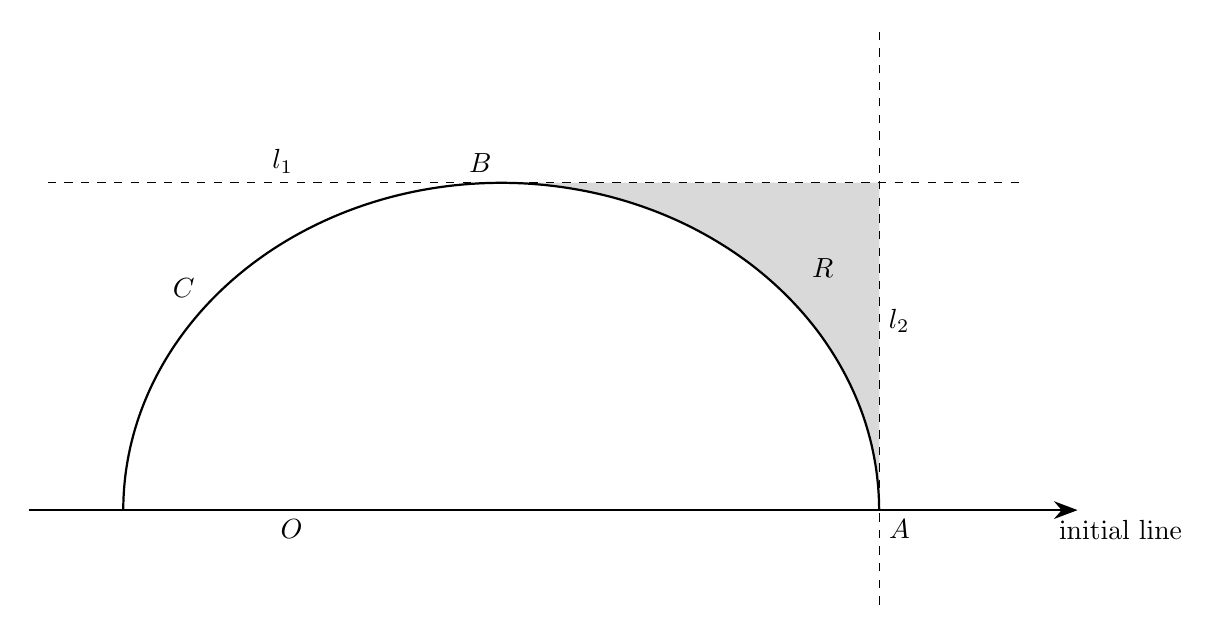
\begin{tikzpicture}[scale=1.2]
\def\a{6}
\def\thB{60}
\pgfmathsetmacro{\xA}{\a}
\pgfmathsetmacro{\rB}{\a/(2-cos(\thB))}
\pgfmathsetmacro{\xB}{\rB*cos(\thB)}
\pgfmathsetmacro{\yB}{\rB*sin(\thB)}
\pgfmathsetmacro{\xC}{\a*cos(118)/(2-cos(118))}
\pgfmathsetmacro{\yC}{\a*sin(118)/(2-cos(118))}

\coordinate (O) at (0,0);
\coordinate (A) at (\xA,0);
\coordinate (B) at (\xB,\yB);
\coordinate (T) at (\xA,\yB);
\coordinate (Rpos) at ($ (B)!0.6!(T) + (1,-0.9) $);

\fill[gray!30] (B) -- (T) -- (A) --
  plot[smooth, samples=120, domain=0:\thB, variable=\t]
    ({\a*cos(\t)/(2-cos(\t))},{\a*sin(\t)/(2-cos(\t))})
  -- cycle;

\draw[dashed] (-2.8,\yB) -- (7.5,\yB);
\draw[dashed] (\xA,-1) -- (\xA,5.1);
\draw[-{Stealth[length=3mm]}, thick] (-3,0) -- (8.1,0);

\draw[thick]
  plot[smooth, samples=200, domain=0:180, variable=\t]
    ({\a*cos(\t)/(2-cos(\t))},{\a*sin(\t)/(2-cos(\t))});

\node[below left] at (O) {$O$};
\node[below right] at (A) {$A$};
\node[above left] at (B) {$B$};
\node[above left] at (\xC,\yC) {$C$};
\node at (Rpos) {$R$};
\node[above left] at (-0.1,\yB) {$l_1$};
\node[right] at (\xA,2.0) {$l_2$};
\node[below right] at (7.8,0) {initial line};
\end{tikzpicture}
\end{figure}


The figure above shows a sketch of the curve $C$ with equation
\[
r = \frac{6}{2 - \cos \theta} \qquad 0 \leq \theta \leq \pi
\]
\\
Given that $C$ meets the initial line at the point $A$, as shown in the figure above \\
\begin{enumerate}[label=\textbf{(\alph*)}]
  \item write down the polar coordinates of $A$. \marks{1} \\
\end{enumerate}
The line $\ell_1$, also shown in the figure above, is the tangent to $C$ at the point $B$ and is parallel to the initial line. \\
\begin{enumerate}[label=\textbf{(\alph*)}, resume]
  \item Use calculus to determine the polar coordinates of $B$. \marks{4} \\
\end{enumerate}
The line $\ell_2$, also shown in the figure above, is the tangent to $C$ at $A$ and is perpendicular to the initial line. \\

The region $R$, shown shaded in the figure above, is bounded by $C$, $\ell_1$ and $\ell_2$. \\
\begin{enumerate}[label=\textbf{(\alph*)}, resume]
  \item By first obtaining a Cartesian equation for $C$, use algebraic integration to find the exact area of $R$, giving your answer in the form $\sqrt{3}(p + q\pi)$ where $p$ and $q$ are constants to be determined. \marks{8} \\
\end{enumerate}

\vspace*{10pt}

\begin{tcolorbox}[colback=white, colframe=scarlet, title={\textbf{Solution}}, breakable, grow to left by=6mm, grow to right by=10mm]
\begin{enumerate}[label=\textbf{(\alph*)}]
\item On the initial line, \(\theta=0\).

\[
r=\frac{6}{2-\cos 0}=\frac{6}{2-1}=6
\]

So the polar coordinates of \(A\) are \((6,0)\).

\item Using
\[
x=r\cos\theta,\qquad y=r\sin\theta
\]
we have
\[
x=\frac{6\cos\theta}{2-\cos\theta},
\qquad
y=\frac{6\sin\theta}{2-\cos\theta}
\]

For a tangent parallel to the initial line, we need
\[
\frac{\mathrm{d}y}{\mathrm{d}x}=0
\]
and
\[
\frac{\mathrm{d}y}{\mathrm{d}x}
=
\frac{\dfrac{\mathrm{d}y}{\mathrm{d}\theta}}{\dfrac{\mathrm{d}x}{\mathrm{d}\theta}}
\]

Now differentiate \(x\) and \(y\) with respect to \(\theta\).

\begin{align*}
\frac{\mathrm{d}x}{\mathrm{d}\theta}
&=
\frac{(-6\sin\theta)(2-\cos\theta)-6\cos\theta(\sin\theta)}{(2-\cos\theta)^2} \\
&=
\frac{-12\sin\theta+6\sin\theta\cos\theta-6\sin\theta\cos\theta}{(2-\cos\theta)^2} \\
&=
\frac{-12\sin\theta}{(2-\cos\theta)^2}
\end{align*}

For \(0<\theta<\pi\), \(\sin\theta\neq 0\), so \(\dfrac{\mathrm{d}x}{\mathrm{d}\theta}\neq 0\).  
Hence a horizontal tangent occurs when
\[
\frac{\mathrm{d}y}{\mathrm{d}\theta}=0
\]

Now
\begin{align*}
\frac{\mathrm{d}y}{\mathrm{d}\theta}
&=
\frac{6\cos\theta(2-\cos\theta)-6\sin^2\theta}{(2-\cos\theta)^2} \\
&=
\frac{12\cos\theta-6\cos^2\theta-6\sin^2\theta}{(2-\cos\theta)^2} \\
&=
\frac{12\cos\theta-6(\cos^2\theta+\sin^2\theta)}{(2-\cos\theta)^2} \\
&=
\frac{12\cos\theta-6}{(2-\cos\theta)^2} \\
&=
\frac{6(2\cos\theta-1)}{(2-\cos\theta)^2}
\end{align*}

So
\[
\frac{\mathrm{d}y}{\mathrm{d}\theta}=0
\quad\Rightarrow\quad
2\cos\theta-1=0
\quad\Rightarrow\quad
\cos\theta=\frac12
\]

Since \(0\leq \theta\leq \pi\),
\[
\theta=\frac{\pi}{3}
\]

Then
\[
r=\frac{6}{2-\cos\left(\frac{\pi}{3}\right)}
=
\frac{6}{2-\frac12}
=
\frac{6}{\frac32}
=4
\]

So the polar coordinates of \(B\) are
\[
(4,\tfrac{\pi}{3})
\]

\item Start with the polar equation
\[
r=\frac{6}{2-\cos\theta}
\]

Rearranging,
\[
r(2-\cos\theta)=6
\]

Using \(x=r\cos\theta\), this gives
\[
2r-x=6
\]

Also, since \(r^2=x^2+y^2\),
\[
2r=x+6
\]

Squaring both sides,
\begin{align*}
4r^2&=(x+6)^2 \\
4(x^2+y^2)&=x^2+12x+36 \\
3x^2+4y^2-12x-36&=0
\end{align*}

Complete the square in \(x\):
\begin{align*}
3(x^2-4x)+4y^2&=36 \\
3\bigl((x-2)^2-4\bigr)+4y^2&=36 \\
3(x-2)^2+4y^2&=48
\end{align*}

So a Cartesian equation for \(C\) is
\[
3(x-2)^2+4y^2=48
\]

Since \(0\leq \theta\leq \pi\), the curve lies above the \(x\)-axis, so
\[
y=\frac{\sqrt{3}}{2}\sqrt{16-(x-2)^2}
\]

Now find the bounding lines.

At \(A=(6,0)\), the tangent \(l_2\) is perpendicular to the initial line, so it is vertical:
\[
l_2:\ x=6
\]

From part (b), \(B=(4,\pi/3)\), so in Cartesian coordinates
\[
x=4\cos\frac{\pi}{3}=2,
\qquad
y=4\sin\frac{\pi}{3}=2\sqrt{3}
\]

Since \(l_1\) is parallel to the initial line, it is horizontal:
\[
l_1:\ y=2\sqrt{3}
\]

Hence the area of \(R\) is
\[
\int_{2}^{6}\left(2\sqrt{3}-\frac{\sqrt{3}}{2}\sqrt{16-(x-2)^2}\right)\,\mathrm{d}x
\]

So
\begin{align*}
\text{Area}(R)
&=
\int_{2}^{6}2\sqrt{3}\,\mathrm{d}x
-
\frac{\sqrt{3}}{2}\int_{2}^{6}\sqrt{16-(x-2)^2}\,\mathrm{d}x \\
&=
8\sqrt{3}
-
\frac{\sqrt{3}}{2}\int_{2}^{6}\sqrt{16-(x-2)^2}\,\mathrm{d}x
\end{align*}

Let
\[
u=x-2
\]
Then when \(x=2\), \(u=0\), and when \(x=6\), \(u=4\). So
\[
\text{Area}(R)
=
8\sqrt{3}
-
\frac{\sqrt{3}}{2}\int_{0}^{4}\sqrt{16-u^2}\,\mathrm{d}u
\]

Now use \(u=4\sin t\). Then
\[
\mathrm{d}u=4\cos t\,\mathrm{d}t
\]
and the limits become \(t=0\) to \(t=\frac{\pi}{2}\).

\begin{align*}
\int_{0}^{4}\sqrt{16-u^2}\,\mathrm{d}u
&=
\int_{0}^{\pi/2}\sqrt{16-16\sin^2 t}\,(4\cos t)\,\mathrm{d}t \\
&=
\int_{0}^{\pi/2}4\cos t\cdot 4\cos t\,\mathrm{d}t \\
&=
16\int_{0}^{\pi/2}\cos^2 t\,\mathrm{d}t \\
&=
16\int_{0}^{\pi/2}\frac{1+\cos 2t}{2}\,\mathrm{d}t \\
&=
8\int_{0}^{\pi/2}(1+\cos 2t)\,\mathrm{d}t \\
&=
8\left[t+\frac12\sin 2t\right]_{0}^{\pi/2} \\
&=
8\left(\frac{\pi}{2}\right) \\
&=
4\pi
\end{align*}

Therefore
\begin{align*}
\text{Area}(R)
&=
8\sqrt{3}-\frac{\sqrt{3}}{2}(4\pi) \\
&=
8\sqrt{3}-2\pi\sqrt{3} \\
&=
\sqrt{3}(8-2\pi)
\end{align*}

So the exact area is
\[
\sqrt{3}(8-2\pi)
\]
and therefore
\[
p=8,\qquad q=-2
\]
\end{enumerate}
\end{tcolorbox}


\end{enumerate}
\end{document}
